
\subsubsection{07.10.14}

\begin{enumerate}
	\item Время начала и окончания собрания:\newline
	17:00 - 21:30
	\item Цели собрания:\newline
	\begin{enumerate}
	  \item Написать программу для управления роботом с джойстика.\newline
	  
	  \item Начать создание подъемника для шаров.\newline
	  
    \end{enumerate}
	\item Проделанная работа:\newline
	\begin{enumerate}
	  \item Сегодня было реализовано управление роботом с помощью джойстика. Управление моторами осуществлялось с помощью левого аналогового датчика. В ходе испытаний было выяснено, что когда на моторы подается малый ток, они не могут провернуться, и издают громкий неприятный звук, вероятно свидетельствующий о том, что они работают на износ. В связи с этим было решено поставить ограничение на подачу моторам слишком слабого сигнала.\newline
      
      \item  Для того, чтобы поднимать корзину на 120 см, было решено собрать две направляющих, каждая из которых состоит из четырех мебельных реек, двух по 30 см и двух по 35 см. Таким образом, рабочая высота составила 130 см. Направляющие были установлены на робота, однако каким образом будет реализован механизм для их раздвигания пока неизвестно.\newline
      
      \begin{figure}[H]
      	\begin{minipage}[h]{0.31\linewidth}
      		\center {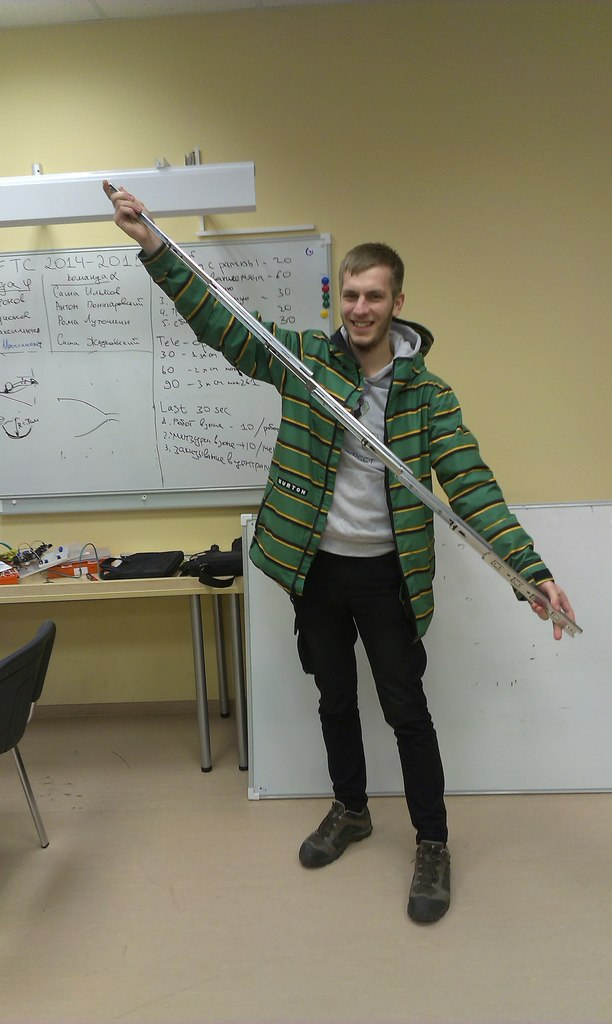
\includegraphics[height=0.9\measurepage]{days/images/Length1}}
      	\end{minipage}
      	\hfill
      	\begin{minipage}[h]{0.31\linewidth}
      		\center{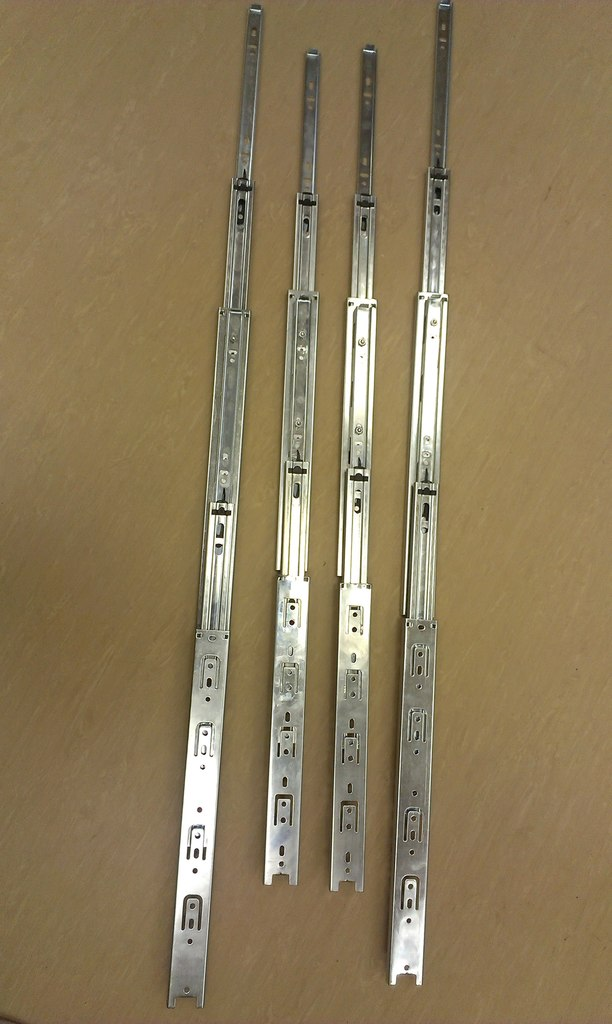
\includegraphics[height=0.9\measurepage]{days/images/Length2}}
      	\end{minipage}
      	\hfill
      	\begin{minipage}[h]{0.31\linewidth}
      		\center{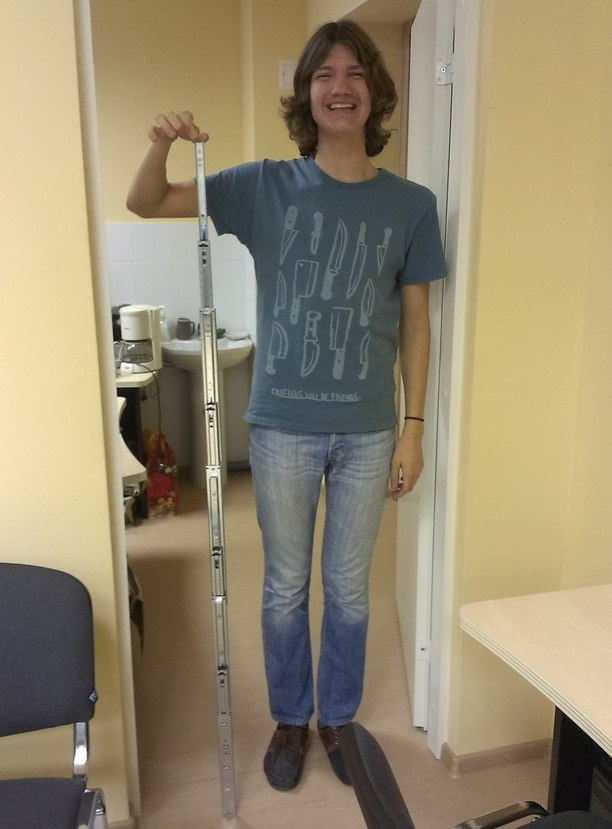
\includegraphics[height=0.9\measurepage]{days/images/Length3}}
      	\end{minipage}
      	\caption{Направляющие для подъемника}
      \end{figure}
      
      \item Поскольку во внутренней части робота оставалось много свободного пространства, было решено установить подъемник шаров в центральной части робота, а управляющую электронику переместить в заднюю часть робота и закрепить ее там для предотвращения ее повреждения расположенным рядом механизмом подъема шаров. В передней части робота было оставлено место для ковша. \newline
       
      \item Поскольку ковш будет опускаться внутри робота, она будет защищена от столкновений с другими роботами. Но в таком случае встает вопрос о том, как мячи будут попадать в ковш, если она будет располагаться внутри робота. Для решения данной проблемы было решено увеличить расстояние между полом и нижней частью передней балки каркаса до 7 см, чтобы в него мог пройти большой шарик. Этого удалось добиться поворотом моторов вокруг своей оси в местах их крепления из положения, в котором вал находится сверху в положение, в котором вал находится сбоку. Кроме того, такое решение позволило отдалить колеса друг от друга, несколько увеличив устойчивость робота.\newline
      
      \begin{figure}[H]
      	\begin{minipage}[h]{1\linewidth}
      		\center{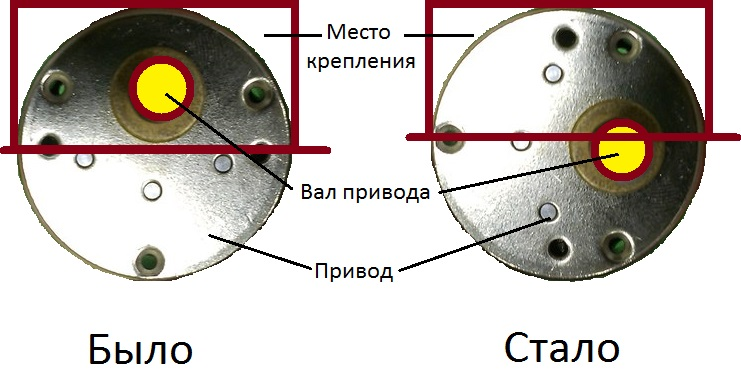
\includegraphics[width=1\linewidth]{days/images/acCxe02qNzs}}
      		\caption{Увеличение клиренса} 
      	\end{minipage}
      \end{figure}
        
      \item Впоследствии в передней части робота было решено установить мягкие щетки, подобные тем, которые устанавливаются на снегоуборочные машины, которые будут вращаться и захватывать мячи. В случае, когда робот собрал максимальное количество шариков, оператор сможет остановить вращение щеток, что не даст другим мячам случайно попасть в ковш.\newline
      
      \begin{figure}[H]
      	\begin{minipage}[h]{0.47\linewidth}
      	    \center{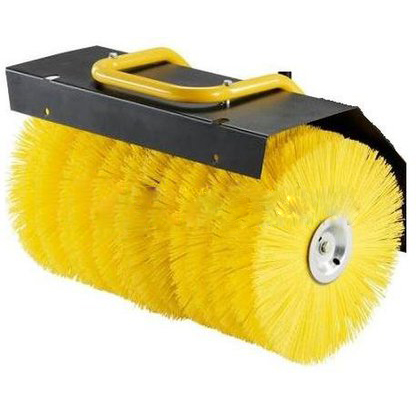
\includegraphics[width=1\linewidth]{days/images/texas_902275600}}
      	\end{minipage}
      	\hfill
      	\begin{minipage}[h]{0.47\linewidth}
      		\center{
\includegraphics[width=1\linewidth]{days/images/missing_image}}
      	\end{minipage}
      	\vfill
      	\begin{minipage}[h]{0.47\linewidth}
      	  \centerВнешний вид
        \end{minipage}
        \hfill
      	\begin{minipage}[h]{0.47\linewidth}
      	  \centerПринцип работы
        \end{minipage}
      	\caption{Идея для захвата мячей}
      \end{figure}
      
    \end{enumerate}
    
	\item Итоги собрания: \newline
	\begin{enumerate}
	  \item  Реализована простейшая программа по управлению роботом, нуждающаяся в доработке.\newline
	  
      \item  Созданы и закреплены на роботе направляющие для подъемника.\newline
      
      \item  Батарея и драйверы моторов надежно зафиксированы на роботе, блок NXT не был закреплен, поскольку его периодически требуется вынимать для замены аккумулятора.\newline
      
      \item  Увеличен клиренс робота.\newline
      
    \end{enumerate}
    
	\item Задачи для последующих собраний:\newline
	\begin{enumerate}
	  \item Доработать программу управления роботом.\newline
	  
	  \item Реализовать управление роботом по Bluetooth.\newline
	  
	  \item Разработать механизм раздвигания направляющих.\newline

    \end{enumerate}     
\end{enumerate}

\fillpage
